\subsubsection*{Youtube-8M}
YouTube-8M คือชุดข้อมูลวิดีโอที่เป็น multi-label ที่มีจำนวนวิดีโอเยอะที่สุด ซึ่งมีจำนวนมากถึง 8 ล้านวิดีโอ(ในปี 2016) โดยมีจุดมุ่งหมายหลักในการอธิบายธีมหลักของวิดีโอด้วยคำสั้นๆ เช่น ถ้าวิดีโอนั้นเป็นวิดีโอที่มี มนุษย์กำลังปั่นจักรยานบนถนนดินกับหน้าผา ชุดข้อมูลนี้จะอธิบายวิดีโอนี้ว่า mountain biking ซึ่งทำให้ YouTube-8M แตกต่างจากชุดข้อมูลวิดีโออื่นๆส่วนใหญ่ที่จะเน้น action หรือ activity ของมนุษย์ ซึ่งข้อมูลเชิงสถิติจะเป็นดังตารางที่ 1

\begin{figure}[!ht]
	\centering
	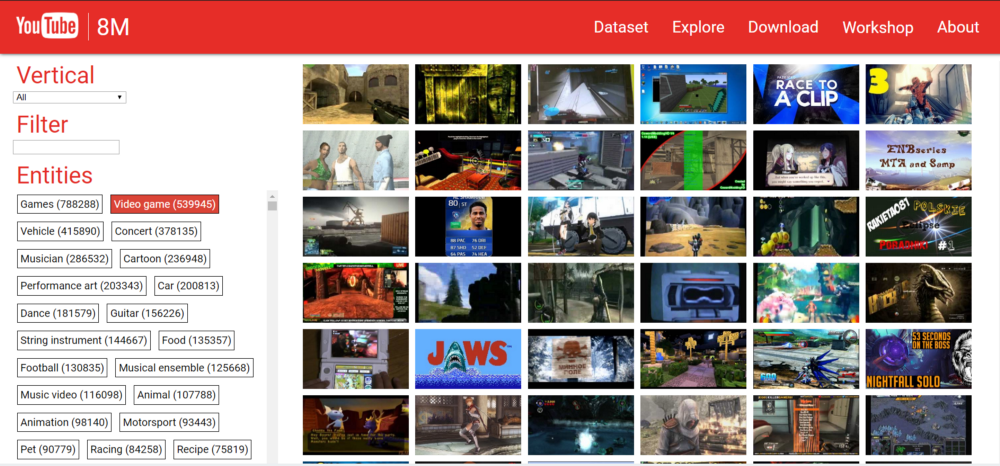
\includegraphics[width=1\textwidth]{chapter2/images/youtube-8m.png}
		\caption{ตัวอย่าง catagories ต่างๆของ YouTube-8M}
    	\label{fig:youtube-8m}
\end{figure}

\begin{table}[!ht]
\begin{tabular}{|c|c|c|c|}
		\hline
		{Number of video}&{Class of video}&{Avg. length of each video(s.)}&{Avg. class of video}				\\
		\hline
		8,264,650		& 4800		& 229.6		& 1.8											\\
		\hline
	\end{tabular}
	\caption{ข้อมูลเชิงสถิติของ YouTube-8M}
	\label{tab: ข้อมูลเชิงสถิติของ YouTube-8M}
\end{table}

\subsubsection*{1. วิธีการรวบรวมข้อมูล}
การเก็บข้อมูลของ YouTube-8M นั้นใช้เครื่องมือที่ชื่อว่า YouTube annotation system ในการเก็บรวบรวมข้อมูลโดยอาศัยผังความรู้(knowledge graph)ของ Google ในการค้นหาและรวบรวมข้อมูลในฐานข้อมูลของ YouTube
\begin{enumerate}
	\setlength\itemsep{-0.25em}
	\item กฏในการรวบรวมข้อมูลดังนี้
	\begin{enumerate}
		\setlength\itemsep{-0.25em}
		\item ทุกๆ หัวข้อต้องเป็นรูปธรรม
		\item ในแต่ละหัวข้อต้องมีจำนวนวิดีโอไม่น้อยกว่า 200 วิดีโอ
		\item ความยาวของวิดีโอต้องอยู่ระหว่าง 120 - 500 วินาที
	\end{enumerate}
หลังจากได้กฏในการรวบรวมข้อมูลแล้ว ขั้นตอนต่อไปคือการสร้างคำศัพท์(vocabulary)ที่ใช้ในการค้นหาข้อมูลวิดีโอจากใน YouTube 
	\item ขั้นตอนในการสร้างคำศัพท์มีดังนี้
	\begin{enumerate}
		\setlength\itemsep{-0.25em}
		\item กำหนด whitelist หัวข้อที่เป็นรูปธรรมมา 25 ชนิด เช่น game เป็นต้น
		\item กำหนด blacklist หัวข้อที่คิดว่าไม่เป็นรูปธรรมไว้ เช่น software เป็นต้น
		\item รวบรวมหัวข้อที่มีอยู่ใน whitelist อย่างน้อย 1 หัวข้อ และต้องไม่มีอยู่ใน blacklist ซึ่งจะทำให้ได้หัวข้อที่ต้องการมาประมาณ 50,000 หัวข้อ
		\item จากนั้นใช้ผู้ประเมินจำนวน 3 คน ในการคัดหัวข้อที่คิดว่าเป็นรูปธรรม และสามารถจดจำหรือเข้าใจได้ง่ายโดยไม่ต้องเชี่ยวชาญในด้านนั้นๆ ซึ่งผู้ประเมิน ก็จะมีคำถามว่า “ มันยากขนาดไหนถึงจะระบุได้ว่ามีหัวข้อดังกล่าวอยู่ในรูปหรือวิดีโอ โดยใช้เพียงแค่การมองรูปภาพเท่านั้น? ” โดยแบ่งเป็นระดับดังนี้
		\begin{enumerate}
			\setlength\itemsep{-0.25em}
			\item บุคคลทั่วไปสามารถเข้าใจได้
			\item บุคคลทั่วไปที่ผ่านการอ่านบทความที่เกี่ยวข้องมาแล้วสามารถเข้าใจได้
			\item ต้องเชี่ยญในด้านใดซักด้านจึงจะเข้าใจได้
			\item เป็นไปไม่ได้ ถ้าไม่มีความรู้ที่ไม่ได้เป็นรูปธรรม
			\item ไม่เป็นรูปธรรม
		\end{enumerate}
		\item หลังจากคำถามข้างบนและการให้คะแนน จะทำการเก็บไว้เฉพาะหัวข้อที่มีคะแนนเฉลี่ยมากที่สุดอยู่ที่ประมาณ 2.5 คะแนนเท่านั้น
		\item ทำให้สุดท้ายเหลือเพียงประมาณ 10,000 หัวข้อที่สามารถใช้ได้
		\item หลังจากได้หัวข้อที่คิดว่าเป็นรูปธรรมแล้วก็นำไปค้นหาและรวบรวมด้วย YouTube annotation system โดยมีขั้นตอนดังนี้
		\begin{enumerate}
			\setlength\itemsep{-0.25em}
			\item สุ่มเลือกวิดีโอมา 10 ล้านวิดีโอ พร้อมกับหัวข้อของวิดีโอ โดยใช้กฏที่กำหนดไว้ เอาหัวข้อที่มีจำนวนวิดีโอน้อยกว่า 200 วิดีโอออก
			\item ทำให้เหลือจำนวนวิดีโออยู่ 8,264,650 วิดีโอ
			\item แยกออกเป็น 3 ส่วน Train set, Validate set และ Test set ในอัตราส่วน 70:20:10 ตามลำดับ
		\end{enumerate}
	\end{enumerate}
\end{enumerate}

เนื่องจากชุดข้อมูลนี้มีขนาดมากกว่า 100 Terabytes และมีความยาวรวมประมาณ 500,000 ชั่วโมง ทำให้การจะใช้คอมพิวเตอร์ทั่วไปเปิดอาจจะใช้เวลานานถึง 50 ปี ทำให้ Google ทำการลดขนาดของข้อมูลลงโดยมีขั้นตอนดังนี้
\begin{figure}[!ht]
	\centering
	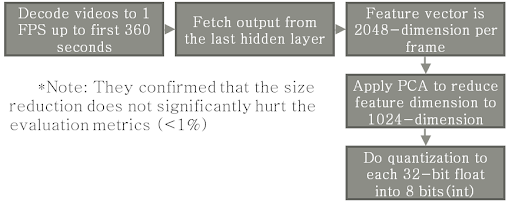
\includegraphics[width=1\textwidth]{chapter2/images/decrease_data.png}
		\caption{ขั้นตอนกระบวนการการลดขนาดของชุดข้อมูลให้สามารถใช้งานได้ง่ายยิ่งขึ้น}
    	\label{fig:decrease_data}
\end{figure}




\subsubsection*{2. การทดลองและวิเคราะห์ผล}
ในบทความ \footnote{YouTube-8M,https://arxiv.org/pdf/1609.08675.pdf} นั้นได้นำเสนอวิธีการในการจัดการข้อมูลซึ่งแบ่งเป็น 2 รูปแบบตามลักษณะของข้อมูลที่ใช้ และอัลกอริทึมหรือเทคนิคที่ใช้ในการสร้างโมเดล ดังนี้
\begin{enumerate}
	\setlength\itemsep{-0.25em}
	\item คุณลักษณะระดับเฟรม (Frame-level feature)
	\begin{enumerate}
		\setlength\itemsep{-0.25em}
		\item Frame-Level Models and Average Pooling
		\\ อันดับแรกเนื่องจากว่าชุดข้อมูลนี้ไม่มีการระบุหัวข้อในระดับเฟรม จึงใช้วิธีการนำหัวข้อในระดับวิดีโอ มากำหนดให้กับทุกๆเฟรมในวิดีโอแทน จากนั้นสุ่มเฟรมมา 20 เฟรมในแต่ละวิดีโอ ทำให้มีเฟรมถึง 120 ล้านเฟรม ซึ่งในแต่ละหัวข้อ $e$ ทำให้มี $(x_{i}, y_{i}^{e})$ 120 ล้านคู่ โดยที่ $x_{i} \epsilon  R^{1024}$ คือ คุณลักษณะที่ได้มาจาก hidden layer สุดท้ายก่อนจะเป็น fully connected และ $y_{i}^{e} \epsilon  0,1$ คือหัวข้อสำหรับหัวข้อ $e$ ของตัวอย่างที่ $i^{th}$ แล้วสร้างโมเดลทั้งหมด 4,800 โมเดลที่เป็นโมเดลแบบ one vs all classifier และเป็นอิสระต่อกันสำหรับแต่ละหัวข้อ และเนื่องจากการประเมินผลนั้นมีพื้นฐานมาจากหัวข้อในระดับวิดีโอ ทำให้ต้องทำการรวมความน่าจะเป็นของแต่ละหัวข้อในระดับเฟรมไปเป็นความน่าจะเป็นในระดับวิดีโอ โดยใช้การเฉลี่ยค่าความน่าจะเป็นทั้งหมดในหัวข้อนั้นๆ และใช้ average pooling เพื่อลดผลจากการตรวจจับความผิดปกติและความโดดเด่นของข้อมูลของแต่ละหัวข้อภายในวิดีโอ
		
		\item Deep Bag of Frames (DBoF) Pooling
		\begin{figure}[!ht]
			\centering
			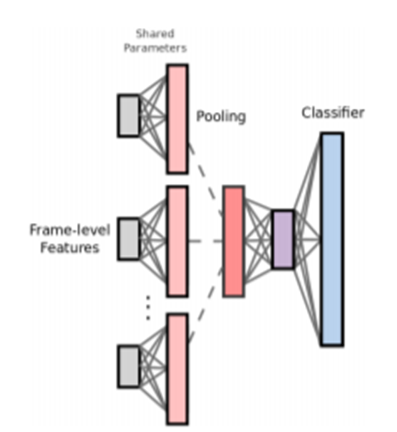
\includegraphics[width=0.5\textwidth]{chapter2/images/DBoF.png}
				\caption{โครงสร้างของโมเดล DBoF}
    			\label{fig:DBoF}
		\end{figure}
		\\ หลักการคล้ายๆกับ Deep Bag of Words โดยที่จะสุ่มเฟรม มา k เฟรม โดยที่แต่ละเฟรมเป็น N dimension input มาผ่าน fully connected ที่มี M units (M > N) และใช้ RELU activations แล้วทำ batch normalization ก่อนจะนำมารวมด้วย max pooling โดยที่ทั้งโครงข่ายใช้ Stochastic  Gradient Descent(SGD) 
		\clearpage
		\item Long short-term memory(LSTM)
		\\ ในบทความ {YouTube-8M,https://arxiv.org/pdf/1609.08675.pdf} นี้ได้ใช้ LSTM แบบเดียวกับของ Beyond Short Snippets: Deep Networks for Video Classification \footnote{AVA,https://arxiv.org/pdf/1705.08421.pdf} แต่เนื่องจาก YouTube-8M นั้นผ่านการทำ preprocess มาแล้วทำให้ไม่สามารถใช้ raw video frame ได้ จึงทำได้เฉพาะ LSTM และ softmax layer เท่านั้น ตามรูปที่ \ref{fig:BSS}
		\begin{figure}[!ht]
			\centering
			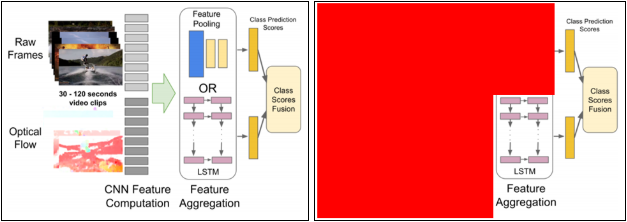
\includegraphics[width=1\textwidth]{chapter2/images/BSS.png}
			\caption{(ซ้าย) โครงสร้างจาก Beyond Short Snippets: Deep Networks for Video Classification, (ขวา) ส่วนที่สามารถใช้งานกับ YouTube-8M ได้}
    		\label{fig:BSS}
		\end{figure}
	\end{enumerate}
	\item คุณลักษณะระดับวิดีโอ (Video-level feature)
	\begin{enumerate}
		\setlength\itemsep{-0.25em}
		\item Video-level representation 
		\\ ในบทความ \footnote{YouTube-8M,https://arxiv.org/pdf/1609.08675.pdf}นี้ได้สำรวจวิธีการแยกเวกเตอร์คุณลักษณะระดับวิดีโอความยาวคงที่จากคุณลักษณะระดับเฟรมซึ่งการทำแบบนี้ทำให้ได้ประโยชน์ 3 ข้อ คือ 1) โมเดลทั่วไปที่ไม่ใช่ neural network สามารถนำไปใช้งานได้  2) ขนาดข้อมูลเล็กลง  3) เหมาะกับการนำไปสร้างโมเดล domain adaptive มากขึ้น
		\begin{enumerate}
			\setlength\itemsep{-0.25em}
			\item First, Second order and ordinal statistic
			\\ จากคุณลักษณะในระดับเฟรม $x_{1:F_{v}}^{v}$ โดยที่ $x_{j}^{v}$ คือคุณลักษณะระดับเฟรมในเฟรมที่ $j$ ของวิดีโอ $v$ และ $F_{v}$ คือจำนวนเฟรมทั้งหมดของวิดีโอ $v$ ทำการหาค่าเฉลี่ย $\mu_{v}$ และส่วนเบี่ยงเบนมาตรฐาน $\sigma_{v}$ พร้อมทั้งดึง ordinal statistics 5 อันดับแรกของแต่ละ dimension K ออกมา $Top_{k}(x^{v}(j)_{1:F_{v}})$ จะทำให้ได้เวคเตอร์คุณลักษณะ(feature-vector) $\varphi_{1:F_{v}}^{v}$ ของวิดีโอเป็นดังนี้ \\
			\centerline{$\varphi_{1:F_{v}}^{v} = \begin{bmatrix}
								\mu_{1:F_{v}}^{v}\\ 
								\sigma_{1:F_{v}}^{v}\\ 
								Top_{k}(x^{v}(j)_{1:F_{v}})
								\end{bmatrix}$}
			\item Feature normalization \\
			ก่อนที่จะทำการสร้าง one vs all classifiers แต่ละตัวนั้นได้ทำ normalization เวกเตอร์คุณลักษณะ $\varphi_{1:F_{v}}^{v}$ จากนั้นนำค่าเฉลี่ย $\mu_{v}$ ออกแล้วใช้ PCA ในการลด มิติของข้อมูล ซึ่งการทำแบบนี้นั้นทำให้การสร้างโมเดลเป็นไปได้เร็วขึ้น
		\end{enumerate}
		โดยการสร้างโมเดลด้วย video-level presentation นั้น บทความ \footnote{YouTube-8M,https://arxiv.org/pdf/1609.08675.pdf} นี้ได้หยิบมาทดสอบ 3 อัลกอริทึม
		\item Model training algorithm approaches 
		\begin{enumerate}
			\setlength\itemsep{-0.25em}
			\item Logistic Regression
			\item Hinge Loss
			\item Mixture of Experts (MoE)
		\end{enumerate}
		\item Evaluation metrics
		\begin{enumerate}
			\setlength\itemsep{-0.25em}
			\item Mean Average Precision (mAP)
			\item Hit@k
			\item Precision at equal recall rate (PERR)
		\end{enumerate}
	\end{enumerate}
	\item Results
	\begin{enumerate}
		\setlength\itemsep{-0.25em}
		\item Baseline on YouTube-8M dataset
\begin{table}[!ht]
\centering
\begin{tabular}{|c|c|c|c|c|}
		\hline
		{Inpute Features}&{Modeling Approach}&{mAP}&{Hit@1}&{(PERR)}\\
		\hline
		Frame-level, $(x_{1:F_{v}}^{v})$	& Logistic + Average		& 11.0		& 50.8		& 42.2					\\
		Frame-level, $(x_{1:F_{v}}^{v})$	& Deep Bag of Frames	& 26.9		& 62.7		& 55.1					\\
		Frame-level, $(x_{1:F_{v}}^{v})$	& LSTM				& 26.6		& 64.5		& 57.3					\\
		\hline
		Video-level, $\mu$					& Hinge loss					& 26.6		& 64.5		& 57.3				\\
		Video-level, $\mu$					& Logistic Regression				& 26.6		& 64.5		& 57.3				\\
		Video-level, $\mu$					& Mixture-of-2-Expert				& 26.6		& 64.5		& 57.3				\\
		Video-level, $\mu ; \sigma ; Top_{5} $	& Mixture-of-2-Expert				& 26.6		& 64.5		& 57.3				\\
		\hline
	\end{tabular}
	\caption{ประสิทธิภาพของโมเดลที่สร้างจาก YouTube-8M ด้วยวิธีต่างๆตามหัวข้อที่ 1 และ 2 โดยแถวที่ 1 คือ frame-level โมเดลและแถวที่ 2 คือ video-level โมเดล}
	\label{tab: ประสิทธิภาพของโมเดลที่สร้างจาก YouTube-8M}
\end{table}
\\
		จากตารางที่ \ref{tab: ประสิทธิภาพของโมเดลที่สร้างจาก YouTube-8M} จะเห็นว่าการทำ video-level features จากการหาค่าเฉลี่ยของ frame-level features แล้วสร้างโมเดลด้วย Hinge loss หรือ โมเดล Logistic Regression นั้นสามารถเพิ่มประสิทธิภาพได้ไม่น้อย และจากการทดลองทำให้เห็นว่า LSTM ที่มีความลึก 2 layers นั้นสามารถทำให้ผลลัพธ์เป็น state-of-the-art ในขณะนั้นได้ เนื่องจากในขณะที่ DBoF นั้นไม่ได้สนใจลำดับของเฟรม แต่ LSTM ใช้ state information เพื่อคงลำดับของเฟรมเอาไว้
\\
\\
		 LSTM นั้นดีที่สุดยกเว้น mAP, เนื่องจาก one-vs-all binary MoE classifier นั้นมีประสิทธิภาพดีกว่า, LSTM สามารถเพิ่มประสิทธิภาพบน Hit@1 และ PERR ได้เนื่องจากความสามารถในการเรียนรู้ความสัมพันธ์ระยะยาวในโดเมนของเวลา
		\clearpage
		\item Transfer learning video-level presentation from YouTube-8M to Sports-1M dataset
\begin{table}[!ht]
\centering
\begin{tabular}{|c|c|c|c|}
		\hline
		{Approach}&{mAP}&{Hit@1}&{(Hit@1)}\\
		\hline
		Logistic Regression ($\mu$)					& 58.0		& 60.1		& 79.6					\\
		Mixture-of-2-Expert ($\mu$)					& 59.1		& 61.5		& 80.4					\\
		Mixture-of-2-Expert ([$\mu ; \sigma ; Top_{5}$		& 61.3		& 63.2		& 82.6					\\
		LSTM									& 66.7		& 64.9		& 85.6					\\
		+Pretrained on YT-8M							& 67.6		& 65.7		& 86.2					\\
		\hline
		Hierarchical 3D Convolution						& -			& 61.0		& 80.0					\\
		Stacked 3D Convolutions						& -			& 61.0		& 85.0					\\
		LSTM with Optical Flow and Pixels				& -			& 73.0		& 91.0					\\
		\hline
	\end{tabular}
	\caption{ประสิทธิภาพของโมเดลเมื่อถูก transfer learning ด้วยชุดข้อมูล Sports-1M โดยใช้ video-level presentation}
	\label{tab: transfer learning}
\end{table}
\\
		จากตารางที่  \ref{tab: transfer learning} จะเห็นว่าโมเดล LSTM ที่ถูก pretrained จาก YouTube-8M นั้นมีประสิทธิภาพที่ดีกว่า ยกเว้น LSTM with Optical Flow and Pixels ที่มีการใช้ข้อมูลการเคลื่อนไหว(optical flow) ในการสร้างโมเดลด้วย
\\
		
		\item Transfer learning video-level presentation from YouTube-8M to ActivityNet dataset
\begin{table}[!ht]
\centering
\begin{tabular}{|c|c|c|c|}
		\hline
		{Approach}&{mAP}&{Hit@1}&{(Hit@1)}\\
		\hline
		Mixture-of-2-Expert ($\mu$)					& 69.1		& 68.7		& 85.4					\\
		+Pretrained PCA on YT-8M						& 74.1		& 72.5		& 89.3					\\
		Mixture-of-2-Expert ([$\mu ; \sigma ; Top_{5}$		& NO			& 74.2		& 72.3					\\
		+Pretrained PCA on YT-8M						& 77.6		& 74.9		& 91.6					\\
		LSTM									& 57.9		& 63.4		& 81.0					\\
		+Pretrained on YT-8M							& 75.6		& 74.2		& 92.4					\\
		\hline
		Ma, Bargal et al.								& 53.8		& -			& -						\\
		Heilbron et al.								& 43.0		& -			& -						\\
		\hline
	\end{tabular}
	\caption{ประสิทธิภาพของโมเดลเมื่อถูก transfer learning ด้วยชุดข้อมูล ActivityNet โดยใช้ video-level presentation}
	\label{tab: transfer learning ActivityNet}
\end{table}
\\
		จากตารางที่ \ref{tab: transfer learning ActivityNet} จะเห็นว่าโมเดลที่ถูก pretrained จาก YouTube-8M นั้นมีประสิทธิภาพที่ดีขึ้นมากเมื่อเทียบกับ benchmark ก่อนหน้า
	\end{enumerate}
\end{enumerate}

\subsubsection*{3. ปัญหาที่พบ}
เนื่องจากว่า YouTube-8M นั้นมีจำนวนข้อมูลที่เยอะมาก ทำให้ไม่สามารถตรวจสอบได้ทั้งหมดว่า ground-truth ของแต่ละวิดีโอนั้นมีความถูกต้องมากน้อยขนาดไหน ทำให้อาจเกิดข้อผิดพลาดได้ (ปัจจุบัน ปี 2019 YouTube-8M ได้มีการตรวจสอบข้อมูลอีกครั้ง เพื่อเพิ่มประสิทธิภาพของชุดข้อมูลซึ่งทำให้ปัจจุบันจำนวนข้อมูล และจำนวน category นั้นจะลดน้อยลงจากข้อมูลที่ใช้อ้างอิงในบทความ \footnote{YouTube-8M,https://arxiv.org/pdf/1609.08675.pdf} ข้างต้นที่ได้กล่าวมา)






